\documentclass[12pt,journal,compsoc]{IEEEtran}

\hyphenation{op-tical net-works semi-conduc-tor}


\usepackage{graphicx}
\usepackage{xspace}
\usepackage{xcolor}
\usepackage{subfig}
\usepackage{amsmath}
\usepackage{amssymb}
\usepackage{algorithm}
\usepackage{algorithmic}
\usepackage{dsfont}
\usepackage{multirow}
\usepackage{tabulary}
\usepackage{dcolumn}
\usepackage{epstopdf}
\usepackage{tabu}
\makeatletter
\DeclareRobustCommand\onedot{\futurelet\@let@token\@onedot}
\def\@onedot{\ifx\@let@token.\else.\null\fi\xspace}

\def\eg{\emph{e.g}\onedot} \def\Eg{\emph{E.g}\onedot}
\def\ie{\emph{i.e}\onedot} \def\Ie{\emph{I.e}\onedot}
\def\cf{\emph{c.f}\onedot} \def\Cf{\emph{C.f}\onedot}
\def\etc{\emph{etc}\onedot} \def\vs{\emph{vs}\onedot}
\def\wrt{w.r.t\onedot} \def\dof{d.o.f\onedot}
\def\etal{\emph{et al}\onedot}
\makeatother

\newtheorem{defi}{\textbf{Definition}}

\begin{document}

\title{Superpixel Gridization via Minimum Topological Discrepancy for Fast Object Localization}

\author{Wei~Feng,~\IEEEmembership{Member,~IEEE,}
        Liang~Li,
        Liang~Wan,~\IEEEmembership{Member,~IEEE,}
        and~Jiawan~Zhang,~\IEEEmembership{Member,~IEEE,}
\IEEEcompsocitemizethanks{\IEEEcompsocthanksitem W. Feng and L. Li are with the Tianjin Key Laboratory of Cognitive Computing and Application, the School of Computer Science and Technology, Tianjin University, Tianjin, China. Email: wfeng@ieee.org, liangli@tju.edu.cn. \protect\\
% note need leading \protect in front of \\ to get a newline within \thanks as
% \\ is fragile and will error, could use \hfil\break instead.
%E-mail: see http://www.michaelshell.org/contact.html
\IEEEcompsocthanksitem L. Wan and J. Zhang (* Corresponding author, Tel: +86-22-87401540) are with the School of Computer Software, Tianjin University, Tianjin, China. Email: \{lwan,jwzhang\}@tju.edu.cn.}% <-this % stops an unwanted space
%\thanks{Manuscript received April 19, 2005; revised December 27, 2012.}}
}

\markboth{IEEE TRANSACTIONS ON PATTERN ANALYSIS AND MACHINE INTELLIGENCE}{W.~Feng \MakeLowercase{et al.}: Dynamic Minimization of Topological Discrepancy for Superpixel Gridization}


\IEEEtitleabstractindextext{%
\begin{abstract}
In computer vision, many algorithms can be significantly accelerated by leveraging the regular grid structure of image pixels. These successful techniques, however, cannot be easily used to handle superpixels (SPs), due to their inherent irregularity in size, shape, and topology. In this paper, we propose a general and tractable criterion, namely minimum topological discrepancy (MTD), to optimally transforming arbitrary SP-graphs into regular grids, thus enabling the usage of various grid-based acceleration techniques at superpixel-level.

In our formulation, the topological discrepancy from an SP-grid to the original SP-graph is measured by both positional and structural discrepancy scores, which respectively reflect the locality deviations from SP regions to regular grid cells and the deviations of pairwise SP connections in the SP-grid to those in the original SP-graph. To minimize the grid topological discrepancy, we present a hybrid dynamic programming approach to efficiently constructing the optimal MTD SP-grid for a given arbitrarily-structured SP-graph, which averagely needs only $0.06s$ for common-sized images. Extensive experiments on object localization show that our MTD SP-grid outperforms state-of-the-art pixel- and superpixel-level alternatives in accuracy, efficiency,  and the capability of handling large-scale images.
\end{abstract}

% Note that keywords are not normally used for peerreview papers.
\begin{IEEEkeywords}
Superpixel gridization, SP-graph, SP-grid, minimum topological discrepancy (MTD), locality deviation, pairwise SP connection deviation, dynamic programming, object localization.
\end{IEEEkeywords}}


\maketitle

\IEEEpeerreviewmaketitle

\section{Introduction}


The rapid increase of images and videos in present cyberworld has made \emph{efficiency} much more important than ever, which together with \emph{accuracy} become two essential marks in measuring the feasibility of computer vision algorithms to handle real-world problems.

Last decades have witnessed a number of successful methods, by leveraging the regular grid structure of image pixels, to achieve significant improvement in speed. Typical methods include the integral image~\cite{ol:tuzel06} and efficient subwindow search~\cite{ol_ref:ess09} in object localization~\cite{ol:tuzel06}\cite{ol_ref:esr09}\cite{ol_ref:fastess09} and tracking~\cite{ol_ref:esr09,int_hist}, dynamic programming in solving variational and low-level vision problems~\cite{dp_ref:dpvar90}\cite{dp_ref:dpsurvy11}, and some practical techniques in fast energy minimization ~\cite{grid_gc}\cite{mrf_ref:felz04}\cite{mrf_ref:hart09}\cite{grid_effgc}.
\if 0 However, these great successes cannot be shared with the recent advances of superpixel-level algorithms and applications \cite{sp_ref:slic12}\cite{seg_ref:felz04}\cite{ps_ref:suppars10}, due to the inherent irregularity of superpixels in sizes, shapes, and more importantly, topology structures.\fi
On the other hand, superpixels have also exhibited great potentials in fast and accurate image analysis. A lot of recent feasible algorithms are based on superpixels (or over-segmented regions) in various vision tasks, \eg cosegmentation~\cite{coseg_ref:rmcoseg12}\cite{coseg_ref:objcoseg12}, image parsing~\cite{ps_ref:suppars10}, object detection~\cite{ps_ref:gould09}\cite{ol_ref:odspl}, and large displacement optic flow~\cite{sp_ref:spflow12}. The popularity of superpixel-level algorithms mainly results from two reasons: (1)~superpixels largely reduce the number of variables that need to be handled, thus can cause apparently better efficiency; (2)~superpixels usually well respect the local image structures, thus may lead to notably better accuracy than pixel-level alternatives~\cite{coseg_ref:rmcoseg12}\cite{coseg_ref:objcoseg12}\cite{ps_ref:gould09}. However, current superpixel-level algorithms cannot share the great success of the mature grid-based acceleration techniques. The major obstacle lies in the topology irregularity of superpixels.

\begin{figure}[t]
    \begin{center}
        %\fbox{\rule{0pt}{2in} \rule{0.9\linewidth}{0pt}}
        \includegraphics[width=1\linewidth]{figs/figure1_v4.eps}
    \end{center} \vspace{-0.2cm}
    \caption{MTD superpixel gridization. (a) Query image (with query object mask in the corner). (b) Pixel-level RC detection~\cite{ol:tuzel06} result. (c) SP-grid generated by SEEDS~\cite{sp_seeds}. (d) Superpixel-level RC detection result via SEEDS SPs. (e) Irregular SP-graph generated by SLIC ~\cite{sp_ref:slic12}. (f-g) The proposed MTD SP-grid. (h) The RC detection result of our MTD SP-grid. In (b), (d) and (h), the $F_1$-measure of detection results and overall running time (including SPs generation, gridization and matching time) are shown on the left-up corner. The images are best viewed in color.} \vspace{-0.5cm}
    \label{fig:motif}
\end{figure}

As shown in Fig.~\ref{fig:motif}(e), superpixels (SPs) generated by grouping similar pixels into perceptually meaningful atomic regions~\cite{seg_ref:sp4seg03}, may have quite different sizes, shapes, and more importantly, topological structures. To unleash the immense potentials of various grid-based acceleration methods at the superpixel-level, we study how to optimally transform arbitrary SP-graphs into regular SP-grids, which we call \emph{superpixel gridization}. The first attempt to the general-purpose superpixel gridization was reported in our previous work~\cite{sp-grid}, which constructs maximum cohesive SP-grids via cascade dynamic programming.
In this paper, we propose a general and tractable criterion, namely \emph{minimum topological discrepancy} (MTD), under which our previous work can be regarded as a special case.

Specifically, we formulate a SP-grid as a regular $4$-connected grid composed of real \emph{SP nodes} and \emph{dummy nodes}. The goodness of a particular gridizing transformation is measured by the overall topological discrepancy from the output SP-grid, \eg Fig.~\ref{fig:motif}(f), to the original SP-graph, \eg Fig.~\ref{fig:motif}(e). In our model, the topological discrepancy function consists of two parts: (1)~\emph{positional discrepancy} $\mathrm{P}(\mathcal{L})$ that reflects the locality deviations from SP regions to the regular grid cells; and (2)~\emph{structural discrepancy} $\mathrm{S}(\mathcal{L})$ that measures the deviations of pairwise SP connections in the SP-grid to those in the original SP-graph. To minimize the grid topological discrepancy, we present a hybrid dynamic programming approach to efficiently constructing the optimal MTD SP-grid for a given arbitrarily-structured SP-graph. First of all, we consider only the unary positional discrepancy $\mathrm{P}(\mathcal{G})$ and use min-cost bipartite graph matching~\cite{dp_ref:dpsurvy11} to obtain a high-quality initial SP-grid. We then conduct cascade dynamic programming to sub-optimally allocate the SP and dummy nodes in each grid column/row by minimizing the overall discrepancy function.

We empirically find that, for images of common size (\eg $800 \times 600$) and fair number of SPs (\eg $100$), our approach averagely needs only $0.06s$ to converge to good MTD SP-grids. We have tested our approach in the task of fast object detection and localization on real-world benchmark dataset and have compared with state-of-the-art pixel-level and superpixel-level alternatives. Extensive experiments validated the superior performance of our approach in both accuracy and efficiency.

%-------------------------------------------------------------------------
\section{Related Work}

\subsection{Grid-based acceleration}
Since image pixels are evenly sampled into a grid structure, a lot of efforts in last decades have been devoted to explore specific algorithms that leverage the simple and regular grid structure to achieve good efficiency and accuracy. One general and widely-used technique is the integral image ~\cite{ol:tuzel06} that enables fast $\mathrm{O}(1)$ sum evaluation of arbitrary rectangles in an image, thus making brute-force searching based object detection and segmentation practical ~\cite{ol:tuzel06,int_hist}. Another famous grid-based acceleration is efficient subwindow search (ESS) that parameterizes a rectangle with $4$ parameters and uses a branch-and-bound scheme to rapidly seek the target region of interest ~\cite{ol_ref:ess09,ol_ref:esr09,ol_ref:fastess09}. Recently, dynamic programming is found to be applicable in solving general labeling problems, given the hidden variables are grid-structurally correlated ~\cite{dp_label}. Before that, DP has already been used in solving many variational and low-level vision problems ~\cite{dp_ref:dpvar90,dp_ref:dpsurvy11}. Besides, there are a number of particular techniques that can be used to apparently speed-up some popular energy minimization algorithms, \eg s-t graph cuts ~\cite{grid_gc,grid_effgc} and efficient BP ~\cite{mrf_ref:felz04}.
\if 0 Moreover, the grid structure is also useful in computer graphics to accelerate bilateral filtering ~\cite{grid_jbf} and ray tracing ~\cite{LD08CFRGRT}. \fi

\subsection{Regular and near-regular SPs}
The notion of superpixels originates from the over-segmented homogeneous subregions in an image, \eg EGS ~\cite{seg_ref:felz04}. Hence, SPs of an image usually form an irregular graph, with the boundaries well-aligned to image edges. Because of this, SPs are widely used by many recent algorithms in solving various vision problems, such as object segmentation and detection ~\cite{coseg_ref:rmcoseg12,coseg_ref:objcoseg12,ps_ref:gould09,ol_ref:odtip15,ol_ref:odspl}, image parsing ~\cite{ps_ref:suppars10}, and large displacement optic flow ~\cite{sp_ref:spflow12}. These algorithms have shown the large potentials of superpixel-level processing in achieving higher efficiency and accuracy than pixel-level alternatives. Recently, researchers start to realize the importance of SP regularities ~\cite{sp_ref:Fu14,sp_grid:Neubert16}. Typical regular and near-regular SP generation methods include SLIC ~\cite{sp_ref:slic12}, TurboPixel ~\cite{sp_ref:turbosp09}, SuperLattice ~\cite{sp_ref:splattice08}, LatticeCut ~\cite{sp_ref:latticut10}, SEEDS ~\cite{sp_seeds} and LSC ~\cite{sp_ref:splsc}. Among all these methods, SLIC, LSC and TurboPixel can only produce near-regular SPs, SuperLattice and LatticeCut need pre-computed image edge maps as guidance, only SEEDS can independently produce strict SP-grids without extra help.

The first attempt to converting arbitrary SP-graphs into regular SP-grids was proposed in our previous work ~\cite{sp-grid}. After introducing dummy nodes with position-taking function only, we constructed an optimal SP-grid via maximizing the SP-grid coherence, which is defined as the sum of edge weights, with SP locality and appearance encoded, along all direct paths connecting any two nearest neighbouring real nodes in the grid. As discussed later, it can be regarded as a special case of the MTD criterion proposed in this paper.

\if 0
Additionally, few existing superpixel generation methods discuss how to directly apply the regular or near-regular structure to achieve better performance.
\fi

\subsection{Object detection and localization}
Sliding window search is a classical way and has been well studied in object detection and localization ~\cite{learning_localize,ol_ref:Gonzalez_15,ol_ref:Zhang16}. Most sliding window based algorithms seek an optimal bounding box to localize the query object in the target image, by minimizing some proper distance function. Recently, region covariance (RC) searching ~\cite{ol:tuzel06} and efficient subwindow search (ESS) ~\cite{ol_ref:ess09,ol_ref:esr09,ol_ref:fastess09} are two types of successful methods in quickly detecting and localizing complex objects in large-scale images. In our experiments, we have tested the proposed approach and several state-of-the-art pixel- and superpixel-level alternatives in the framework of RC searching.


%-------------------------------------------------------------------------
\section{Problem Formulation}

The topology structure of any SPs can be represented as a weighted SP-graph $\mathcal{G} = \langle \mathcal{P}, \mathcal{E}_{\mathcal{P}}, W_{\mathcal{P}} \rangle$, where $\mathcal{P}$ is the set of SPs; $\mathcal{E}_{\mathcal{P}}$ is the set of pairwise SP connections that can be established via proper neighboring or closeness relationships in feature spaces;\footnote{In our experiments, we evaluated four types of SP edges, \ie spatial $n$-connections, $k$nn, $\epsilon$nn, and $L_1$-graph ~\cite{l1graph10}. See Sec.~\ref{sec:exp} for more details.} and $W_{\mathcal{P}} = [W_{\mathcal{P}}(p,q)]_{p,q=1}^{|\mathcal{P}|}$ is the edge weight matrix. Specifically, for two neighboring SPs $p$ and $q$, we set the edge weight $W_{\mathcal{P}}(p,q)$ as their regularized dissimilarity, given by
\begin{equation} \small
\label{eq:wsp}
\mathrm{dif}(p,q) = \omega_d \mathrm{D}(p, q) - \omega_f \mathrm{F}(p, q) + \omega_e \mathrm{E}(p, q) + C,
\end{equation}
where $\mathrm{D}(p, q)$ is the $L_2$ distance between the regional centroids of $p$ and $q$. $\mathrm{F}(p, q)$ is the SP color similarity measured by the Bhattacharyya coefficient $\mathrm{Ba}(H_p, H_q) = \sum_{b=1}^{8^3} \sqrt{H_p(b) \cdot H_q(b)}$, where $H_p$ and $H_q$ are RGB-channel independently quantized color histograms of $p$ and $q$, respectively.
$\mathrm{E}(p, q)$ is the average gradient magnitude along the common boundary of $p$ and $q$ that measures the inbetween edge strength. Clearly, Eq.~(\ref{eq:wsp}) encourages small SPs similarity if they are spatially far from each other, with dissimilar color histograms and strong inbetween boundary. In Eq.~(\ref{eq:wsp}), non-negative parameters $\omega_d$, $\omega_f$ and $\omega_e$ control the relative influences of spatial distance, feature similarity and edge strength in $\mathrm{dif}(p,q)$, and $C$ is a constant ensuring all edge weights in the graph are non-negative.

\begin{figure}[t]
\begin{center}
%\fbox{\rule{0pt}{2in} \rule{0.9\linewidth}{0pt}}
   %\includegraphics[width=0.99\linewidth]{figs/figure2_v3.eps}
   \includegraphics[width=\linewidth]{figs/figure2_new.eps}
\end{center}
   \caption{Illustration of superpixel gridization by optimally adding dummy nodes. The images are best viewed in color.}
\label{fig:gridize}
\end{figure}

For a given SP-graph $\mathcal{G}$, our objective, \ie \emph{SP gridization}, is to optimally transform $\mathcal{G}$ into a regular $4$-connected grid (or lattice equivalently) $\mathcal{L} = \langle \mathcal{C}, \mathcal{E}_{\mathcal{C}}, W \rangle$, with $\mathcal{C}$ as the set of grid cells and $\mathcal{E}_{\mathcal{C}}$ being the gird edge set. Furthremore, $\mathcal{E}_{\mathcal{C}}$ can be fully determined by 2D-indexed $\mathcal{C}$, equivalently grid height $h$ and width $w$ (\ie the number of cells in a column and a row on the grid). That is, a grid $\mathcal{L}$ can be simply expressed as $\mathcal{L} = \langle \mathcal{C}, (h, w), W \rangle$. As a result, in SP gridization, if considering $h$ and $w$ as manually set parameters, we need to construct two important mapping relationships from $\mathcal{C}$ to $\mathcal{P}$, and from $W$ to $W_{\mathcal{P}}$, respectively. As shown in Fig.~\ref{fig:gridize}, a reasonable and practical way is to add \emph{dummy nodes} (marked as black circles)~\cite{sp-grid} and to explore the \emph{d-linked paths}.

\begin{defi}[d-linked SP nodes \& d-linked path] \label{def:dlink}
In an SP-grid $\mathcal{L}$, two SP nodes $p$ and $q$ are \emph{d-linked} to each other, iff: (1)~they lie in the same column (or row) in the grid; and (2)~all inbetween cells in the column (or row) are filled by dummy nodes. As a special case, two directly connected SP nodes in the grid can also be called d-linked. The path connecting two d-linked SP nodes $p$ and $q$, composed of (if any) only co-column (or co-row) inbetween dummy nodes and $p$, $q$ themselves, is called a \emph{d-linked path}.
\end{defi}

Through gridization, the dummy nodes have two major roles in the SP-grid $\mathcal{L}$: (1)~position taking, which means all grid cells should be filled by either SP nodes $p \in \mathcal{P}$ or dummy nodes $d \in \mathcal{D}$, thus $\mathcal{C} = \mathcal{P} \cup \mathcal{D}$; and (2)~linking SP nodes, which means in SP-grid, the d-linked SP nodes can still be viewed as direct neighbors to each other, thus their dissimilarity should be maintained in the corresponding d-linked path. Accordingly, for any two directly neighbored nodes $i$ and $j$ in SP-grid $\mathcal{L}$, the edge weight can be defined as:
\begin{equation} \label{eq:gridweight} \small
W(i,j) = \left \{
\begin{array}{ll}
\mathrm{dif}(i,j), & \mbox{both } i \mbox{ and } j \mbox{ are SPs}, \\
0, & \mbox{both } i \mbox{ and } j \mbox{ are dummy}, \\
\frac{1}{2} \mathrm{dif}(i,t), & i \mbox{ is SP and } j \mbox{ is dummy}, \\
\frac{1}{2} \mathrm{dif}(t,j), & i \mbox{ is dummy and } j \mbox{ is SP}, \\
\end{array}
\right.
\end{equation}
where $t$ is the SP node d-linked to the SP node $i$ (or $j$), with $j$ (or $i$) as the first or last inbetween dummy node in the d-linked path.

Till now, we can formulate \emph{SP gridization} as the following minimization problem:
\begin{equation} \label{eq:spgrid}
%\hat{\mathcal{L}} = \arg_{\mathcal{L}} \min f(\mathcal{L} | \mathcal{G}, h, w).
\begin{array}{rl}
\hat{\mathcal{L}} & = \arg_{\mathcal{L}} \min f(\mathcal{L} | \mathcal{G}, h, w) \\
& = \arg_{\mathcal{C},W} \min [f_1(\mathcal{C} | \mathcal{P}, h, w) + \alpha f_2(W | W_{\mathcal{P}}) ]
\end{array}
\end{equation}
where $\alpha > 0$ is a weighting parameter controlling the relative importance of $f_1(\cdot)$ and $f_2(\cdot)$, which measures the cost of two mappings from $\mathcal{P}$ to $\mathcal{C}$ and from $W_{\mathcal{P}}$ to $W$, respectively.


%-------------------------------------------------------------------------
\section{Minimizing Grid Topological Discrepancy }

In this section, we introduce a general yet tractable criterion for SP gridization, namely minimum topological discrepancy (MTD), which aims at minimizing the topological deviations from resultant SP-grid $\mathcal{L}$ to the original SP-graph $\mathcal{G}$. Specifically, we consider the positional discrepancy $\mathrm{P}(\mathcal{L})$ and structural discrepancy $\mathrm{S}(\mathcal{L})$, both of which are elaborated detailedly in the following.

\subsection{Positional discrepancy $\mathrm{P}(\mathcal{L})$}

We first consider the \emph{positional discrepancy} $\mathrm{P}(\mathcal{L})$, which reflects the locality deviations from SP regions to the regular grid cells. Let $\mathrm{reg}(p)$ denote the irrgular subregions of SP $p$, and $\mathrm{cell}(i)$ indicate the rectangle region of the $i$-th grid cell. Their positional discrepancy is defined as:
\begin{equation} \label{eq:pidev}
\mathrm{dev}(p, i) = \exp \Big( -\frac{|\mathrm{reg}(p) \cap \mathrm{cell}(i)|}{|\mathrm{cell}(i)|} \Big) + \beta \mathrm{D}(p, i),
\end{equation}
where $|\cdot|$, in this paper, indicates the set cardinality or region area; $\mathrm{D}(p, i)$ is identical to its definition in Eq.~(\ref{eq:wsp}) representing the $L_2$ distance between the regional centroids of SP $p$ and grid cell $i$, $\beta > 0$ is a weighting parameter. $\mathrm{dev}(p, i)$ measures the positional deviation of SP $p$ to grid cell $i$, based on which the overall grid positional discrepancy can be measured by
\begin{equation} \label{eq:posdev}
\mathrm{P}(\mathcal{L}) = \mathrm{f_1}(\mathcal{C} | \mathcal{P}, h, w) = \sum_{p \leftrightarrow i, p \in \mathcal{P}, i \in \mathcal{C}} \mathrm{dev}(p, i),
\end{equation}
where $p \leftrightarrow i$ means SP $p$ is allocated to grid cell $i$. Note that, since $\mathrm{dev}(p, i)$ can be independently evaluated for different SPs, the positional discrepancy $\mathrm{P}(\mathcal{L})$ actually defines unary energy terms in the SP gridization model Eq.~(\ref{eq:spgrid}).

%\begin{figure}[!htb]
%\begin{center}
%\fbox{\rule{0pt}{2in} \rule{0.9\linewidth}{0pt}}
%   %\includegraphics[width=0.8\linewidth]{egfigure.eps}
%\end{center}
%   \caption{Illustration of positional discrepancy between superpixels and the hidden grid cells.}
%\label{fig:posdisc}
%\end{figure}

\subsection{Structural discrepancy $\mathrm{S}(\mathcal{L})$}

For the given SP graph $\mathcal{G}$, the gridization result $\mathcal{L}$ should not severely deviate from the original SP connections, which usually correspond to important image structures. Thus, we define structural discrepancy $\mathrm{S}(\mathcal{L})$ to penalize the pairwise topological differences between SP-grid $\mathcal{L}$ and the original SP-graph $\mathcal{G}$. Specifically, structural discrepancy $\mathrm{S}(\mathcal{L})$ can be measured by
\begin{equation} \label{eq:structdev}
\mathrm{S}(\mathcal{L}) = \mathrm{f_2}(W | W_{\mathcal{P}}) = \sum_{p \in \mathcal{P} \atop q \in \mathcal{P}} | W_{\mathrm{dLink}}(p,q) - W_{\mathcal{P}}(p,q) |,
\end{equation}
where matrix $W_{\mathrm{dLink}}$ is derived from the grid edge weights matrix $W$ and records the dissimilarity of all d-linked SP pairs in the SP-grid $\mathcal{L}$:
\begin{equation} \label{eq:dlmtx}
%W_{\mathrm{dLink}}(p,q)  = \left \{
%\begin{array}{ll}
%0 & p \mbox{ and } q \mbox{ are not d-linked in } \mathcal{L} \\
%\displaystyle \sum_{s \in \mathrm{dPath}(p,q) \atop s \neq p} W(p,s) = \mathrm{dif}(p,q) & \mbox{else}
%\end{array} \right.
W_{\mathrm{dLink}}(p,q)  = \left \{
\begin{array}{ll}
\mathrm{dif}(p,q), & p, q \mbox{ are d-linked in } \mathcal{L} \\
0. & \mbox{else}
\end{array} \right.
\end{equation}
Note, the rationale of $W_{\mathrm{dLink}}$ is guaranteed by the grid edge weights defined in Eq.~(\ref{eq:gridweight}), which ensures $\sum_{s \in \mathrm{dPath}(p,q) \atop s \neq p, s \in \mathcal{P} \cup \mathcal{D}} W(p,s) = \mathrm{dif}(p,q)$ for any two d-linked SPs in $\mathcal{L}$. $\mathrm{dPath}(p,q)$ denotes the d-linked path of $p$ and $q$.

Besides, the structural discrepancy $\mathrm{S}(\mathcal{L})$ defined in Eq.~(\ref{eq:structdev}) can also be viewed as the sum of weights of newly added SP connections in the SP-grid $\mathcal{L}$ and the deleted SP connections from the SP-graph $\mathcal{G}$. See Fig.~\ref{fig:gridize} for illustration. Clearly, $\mathrm{S}(\mathcal{L})$ defines pairwise energy terms in the SP gridization model Eq.~(\ref{eq:spgrid}).

%\begin{figure}[!htb]
%\begin{center}
%\fbox{\rule{0pt}{2in} \rule{0.9\linewidth}{0pt}}
%   %\includegraphics[width=0.8\linewidth]{egfigure.eps}
%\end{center}
%   \caption{Illustration of structural discrepancy from an SP grid to the original SP graph.}
%\label{fig:strucdisc}
%\end{figure}

\subsection{Hybrid dynamic minimization}
%\subsection{Grid topological discrepancy and minimization}

From Eq.~(\ref{eq:posdev}) and (\ref{eq:structdev}), the objective of SP gridization in Eq.~(\ref{eq:spgrid}) becomes:
\begin{equation} \label{eq:Gtd}
\mathrm{Gtd}(\mathcal{L} | \mathcal{G}, h, w) = \mathrm{P}(\mathcal{L}) + \alpha \mathrm{S}(\mathcal{L}).
\end{equation}
For this regularized grid topological discrepancy function, we use a two-step hybrid dynamic programming (DP) approach to obtain the final MTD SP-grid. We first consider only the unary positional discrepancy $\mathrm{P}(\mathcal{L})$ and use min-cost bipartite graph matching to obtain a good initial SP-grid $\mathcal{L}^{(0)}$ ~\cite{dp_ref:dpsurvy11}. See Fig.~\ref{fig:gridize} for an example. Then, we conduct iterative dynamic programming to sub-optimally allocate the SP and dummy nodes in each grid column/row by minimizing the overall discrepancy function $\mathrm{Gtd}(\mathcal{L} | \mathcal{G}, h, w)$.

\subsubsection{Dynamic initialization}
\label{subsec:gridinit}
To initialize, we construct a bipartite graph
$\mathcal{G}_B=\{\mathcal{P}, \mathcal{L}, \mathbf{C}_\mathrm{A}\}$, where the across-cost matrix $\mathbf{C}_\mathrm{A}=(c_{ij})_{|\mathcal{P}|\times |\mathcal{L}|}$
between $\mathcal{P}$ and $\mathcal{L}$ is defined as
\begin{equation}
c_{ij}=\mathrm{dev}(i,j),
\end{equation}
where $i$ denotes the \#i real-node, and $j$ denotes grid cell $j$.
The bipartite graph is illustrated in Fig.~\ref{fig:bg}. Then we adapt the Hungarian algorithm to assign each
cell in $\mathcal{L}$ exactly one SP in $\mathcal{P}$. The cells that do not have corresponding SPs are
assigned dummy nodes.

\begin{figure}[ht]
\includegraphics[width=\linewidth]{figs/bg.eps}
\caption{Illustration of the bipartite graph $\mathcal{G}_B$.}
\label{fig:bg}
\end{figure}

\subsubsection{Iterative dynamic programming}
\label{subsec:gridfine}
Starting from $\mathcal{L}^{(0)}$,  our MTD SP-grid $\mathcal{L}^{\ast}$ is progressively constructed by optimizing its every column/row under the current configurations of other columns/rows. For a particular column/row $\rho$ of current $\mathcal{L}^{\ast}$, we follow the iterative DP procedure~\cite{sp-grid} to update it under the context of current configurations of other columns/rows in $\mathcal{L}^{\ast}$, while strictly maintaining the order of SP nodes in $\rho$:
\begin{equation} \label{eq:dp_S}
\mathrm{S}(k, n) = \max_{k \leq p \leq n+1} [ \mathrm{S}(k-1, p-1) + \mathrm{inc}(p, k, n) ].
\end{equation}
\begin{equation} \label{eq:dp_B}
\mathrm{B_S}(k, n)= \arg\max_{k \leq p \leq n+1} [ \mathrm{S}(k \!-\! 1, p \!-\! 1) + \mathrm{inc}(p, k, n) ].
%\mathrm{B_S}(k, n)= \arg \mathrm{S}(k, n).
\end{equation}
$\mathrm{S}(k, n)$ is the minimum overall grid discrepancy of the related subgraph, asserting the minimum increments caused by allocating $k$ dummy nodes in the first $n$ SP nodes of the current column/row $\rho$. The related subgraph corresponding to such change is composed of all the nodes in the first $n+k$ rows/columns of $\mathcal{L}^{\ast}$ whose states (\ie being either some particular SP node or dummy node) jointly contribute to decreasing $\mathrm{Gtd}(\mathcal{L}^{\ast})$. That is, $\mathrm{S}(k, n)$ is actually the changed component of $\mathrm{Gtd}(\mathcal{L}^{\ast})$.  $\mathrm{inc}(p, k, n)$ denotes the extra discrepancy increments by assigning the \#k dummy node right in front of the \#p real node of $\rho$, which can be calculated as
\begin{equation}\label{eq:dp_inc}
 \mathrm{inc}(p, k, n) = \sum_{i=p}^{n}{Gtd(i,i_r)+Gtd(i,i_l)+Gtd(k_l, k_r)},
\end{equation}
where $i_l$/$k_l$ and $i_r$/$k_r$  are the left-first real nodes and right-first real nodes for \#i/\#k real node of column $\rho$.

\if 0
Iterative dynamic minimization process.



Specifically, we formulate an SP-grid as a regular $4$-connected grid composed of real \emph{SP nodes} and \emph{dummy nodes}. The goodness of a particular gridizing transformation is measured by the overall topological discrepancy from the output SP-grid, \eg Fig.~\ref{fig:motif}(f), to the original SP-graph, \eg Fig.~\ref{fig:motif}(e). In our model, the topological discrepancy function consists of two parts: (1)~\emph{positional discrepancy} $\mathrm{P}(\mathcal{L})$ that reflects the locality deviations from SP regions to the regular grid cells; and (2)~\emph{structural discrepancy} $\mathrm{S}(\mathcal{L})$ that measures the deviations of pairwise SP connections in the SP-grid to those in the original SP-graph. To minimize the grid topological discrepancy, we present a hybrid dynamic programming approach to efficiently constructing the optimal MTD SP-grid for a given arbitrarily-structured SP-graph. First, we consider only the unary positional discrepancy $\mathrm{P}(\mathcal{G})$ and use min-cost bipartite graph matching to obtain an initial SP-grid ~\cite{dp_ref:dpsurvy11}. We then conduct iterative dynamic programming to optimally allocate the SP and dummy nodes in each grid column/row by minimizing the overall discrepancy function. We empirically find that, for images of common size (\eg $800 \times 600$) and fair number of SPs (\eg $100$), our approach averagely needs only $0.06s$ to converge to good MTD SP-grids. We have tested our approach in the task of fast object detection and localization on real-world benchmark dataset and have compared with state-of-the-art pixel-level and superpixel-level alternatives. Extensive experiments validated the superior performance of our approach in both accuracy and efficiency.

\begin{figure}[!htb]
\begin{center}
\fbox{\rule{0pt}{2in} \rule{0.9\linewidth}{0pt}}
   %\includegraphics[width=0.8\linewidth]{egfigure.eps}
\end{center}
   \caption{Dynamic minimization process of the regularized grid topological discrepancy function.}
\label{fig:dp}
\end{figure}
\fi

\subsubsection{The whole algorithm}

Given a SP graph $\mathcal{G}$ whose construction is discussed in subsection~\ref{subsec:spgraph}, we get the initial grid $\mathcal{L}^{(0)}$ from $\mathcal{G}$ via bipartite graph matching introduced in subsection \ref{subsec:gridinit}. Then, we get an optimized grid $\mathcal{L}^{*}$ via minimizing Eq. (\ref{eq:Gtd}) with dynamic programming procedure to refine the dummy nodes location of $\mathcal{L}^{(0)}$ over all columns, as described in subsection \ref{subsec:gridfine}. The whole algorithm is illustrated in Alg. (\ref{alg:hybridDP})

\begin{algorithm}[t]
   \caption{SP-grid via hybrid DP}

   \begin{small}
\begin{algorithmic}[1]
\label{alg:hybridDP}
   \REQUIRE  The superpixel graph $\mathcal{G}$
   \ENSURE  Optimal minimum topological discrepancy grid $\mathcal{L}^*$

   \STATE Compute the edge weight matrix $W$ according to Eq. (\ref{eq:gridweight});
   \STATE Compute the grid positional discrepancy $P(\mathcal{L})$ and the structural discrepancy
          $S(\mathcal{L})$ according Eq. (\ref{eq:dp_S}) and Eq. (\ref{eq:dp_B}) respectively;
   \STATE Construct the bipartite graph $\mathcal{G}_B$ and solve the assignment problem to get the
          initial grid $\mathcal{L}^{(0)}$
   \REPEAT
   \FOR {each column $\rho$ of $\mathcal{G}$}

	   \STATE /* Stage 1: compute $\mathrm{coh}(p, k, n)$ of current column */
	   \FOR {$n=1$ to $|\rho|$, $k=1$ to $m$, $p=k$ to $n+1$}
	       \STATE Compute $\mathrm{inc}(p, k, n)$ as the overall coherence of its correlated subgraph;
	   \ENDFOR
	
	   \STATE /* Stage 2: compute $\mathrm{S}(k, n)$ and $\mathrm{B_S}(k, n)$ */
	   \FOR {$n=1$ to $|\rho|$, $k=1$ to $m$}
		   	\STATE Compute $\mathrm{S}(k, n)$ and $\mathrm{B_S}(k, n)$ using Eqs.~(\ref{eq:dp_S})--(\ref{eq:dp_B});
	   \ENDFOR

       \STATE /* Stage 3: updating $\mathcal{G}^{\ast}$ */
       \STATE Updating $\mathcal{G}^{\ast}$ according to $\mathrm{B_S}(\cdot, \cdot)$;

   \ENDFOR
   \UNTIL{No changing to $\mathcal{G}^{\ast}$};
\end{algorithmic}
   \end{small}
\end{algorithm}

\textbf{Complexity analysis.} The complexity of Hungarian algorithm during initialization is $\mathrm{O}(|\mathcal{P}|^3)$.
The dynamic programming process of optimizing column $\rho$ is $\mathrm{O}(|\rho|^3m)$, where $|\rho|$ is the number of real nodes and $m$
is the number of dummy nodes to be added in the column.
%-------------------------------------------------------------------------
\section{Object Localization via MTD}
\label{sec:gridol}
With the proposed MTD SP-grid method, we thus can transform the grid-based acceleration methods from pixel-level to SP-level to get efficient yet approximate segmentation results for various applications. Here, we focus on the object localization problem , \ie given an object mask in a image, we need to automatically localize the object in another scene with possible huge deformation, scale variation, point view change and so on. We first present four SP graph construction methods as the input of MTD for arbitrary SP segmentation results. Then, we introduce how to use the MTD SP-grid to realize fast yet accuracy object localization with the original pixel-level method, \ie region covariance (RC) detection ~\cite{ol:tuzel06}.
\subsection{SP graph construction}
\label{subsec:spgraph}
For our approach, we have constructed four types of SP-graphs based on the given SP set $\mathcal{P}$ and the edge weight matrix $W_{\mathcal{P}}$:
\begin{itemize}
\item $k$nn. If $p$ is the one of $k$ nearest neighbor of $q$ (according to dif($p,q$) ) and vice verse , then link them.
\item $n$-con. Link the spatially $n$-nearest SPs. Formally, for SP $p$ and $q$ in $\mathcal{P}$, the adjoint matrix $L=(l_{pq})_{|\mathcal{P}|\times|\mathcal{P}|}$ is defined as
    \begin{equation}
l_{pq}=
\left\{
\begin{aligned}
1 &;~~~~ \exists x\in \Omega(I), \{p,q\}\subset\mathcal{P}_{N_x} \\
0 &;~~~~ others
\end{aligned},
\right.
\end{equation}
where $N_x$ is the 4-connected neighborhood of pixel $x$ and $\mathcal{P}_{N_x}$ is the superpixel label set of $N_x$. We regard $p$ and $q$ is connected in $n$-con if and only if $L^n(p,q)\neq 0$;
\item $\epsilon$nn. Link $p$ and $q$ if  dif($p,q$)$<\epsilon$ ;
\item $L_1$ graph. This type of graph is described in ~\cite{l1graph10} and here we introduce it shortly. For SP $p$ in $\mathcal{P}$, we calculate a color histogram with 8 bins per RGB channel $h_p$. For each $p$, we solve the following $\ell_1$ norm minimization to get a sparse representation $h_p$:
\begin{equation}
\min_{\alpha_p}||\alpha_p||_1,~~~~~~s.t.~~~~~h_p=B_p\alpha_p,
\end{equation}
where $B_p=[h_1,\hdots,h_{p-1},h_{p+1},\hdots,h_{\mathcal{P}},E]\in\mathds{R}^{24\times(24+|\mathcal{P}|-1)}$ and $E$ is the identity matrix. The graph is constructed based on the adjacent matrix
\begin{equation*}
L(p,q)=
\left\{
\begin{aligned}
1&;~~~~~\alpha_p(q)\ne 0 ~or~ \alpha_p(q-1)\ne 0\\
0&;~~~~~others
\end{aligned}.
\right.
\end{equation*}
\end{itemize}

For the first 3 graphs, we quantize each of them into 5 levels, namely $k=1, k=5, k=10, k=15, k=25; n=1, n=2, n=3, n=4, n=6$ and $\epsilon=100, \epsilon=200, \epsilon=300, \epsilon=400, \epsilon=500$ \footnote{dif{$(p,q)$} is regularized to [0, 1000]}.
\subsection{MTD SP-grid based object localization}
We extend the pixel level region covariance (RC) detection to superpixel level. Following the notation of ~\cite{ol:tuzel06},
given the input image $I$ and let $F\subset\mathbb{R}^{W\times H\times d}$ be the corresponding feature image:
\begin{equation}
F(x,y) = \phi(I,x,y),
\end{equation}
where $\phi$ can be any mapping of intensity, color, gradients, filter responses or feature statistics. The key of
RC-based object localization is to efficiently compute $F(\mathcal{R})$ for any rectangle $\mathcal{R}$ of $I$
using the integral-image acceleration ~\cite{ol:tuzel06}. Similarly, due to the regular structure of our SP-grid, for
any \emph{logic rectangle} $\mathcal{R}$ on the SP-grid, we can directly use the integral-image technique to compute the
corresponding RC feature of $\mathcal{R}$ in $\mathrm{O}(1)$ time. We need only to define the superpixel-level feature image $F(u,v)$ for an SP-grid $\mathcal{G}=\langle \mathcal{C},\mathcal{E} \rangle$, where $\mathcal{C}=\mathcal{P}\cup\mathcal{D}$ is the vertices set of the grid, $\mathcal{P}$ is the set of real nodes (\ie all SPs) and $\mathcal{D}$ represents all dummy nodes in the grid. The \#$(u,v)$ entry of superpixel-level feature image $F(u,v)$ is defined as the sum of all features of the corresponding image regions:
\begin{equation}
\displaystyle
\mathcal{F}(u,v) =
\left\{
\begin{array}{c l}
\sum\limits_{(x,y) \in \mathcal{V}_{uv}}F(x,y), & \mathcal{C}_{uv} \in \mathcal{P}, \\
0, & \mathcal{C}_{uv}\in\mathcal{D},\\
\end{array}
\right.
\end{equation}
where $\mathcal{V}_{uv}$ denotes the corresponding image region of \#$(u,v)$ superpixel in the SP-Grid, if it is a real node. Clearly, the superpixel-level feature image $F \subset \mathcal{R}^{c \times r \times d}$, where $c$ and $r$ denote the width and height of the SP-grid $\mathcal{G}$, respectively. In our experiments, we used the Lab color, spatial location, and color gradients as the feature.

\section{Experimental Results}
\label{sec:exp}
We validate the effective and efficiency of our MTD SP-grid method via object localization experiments. To get the most sophisticated analysis and the fairest comparison, we first propose to use differential
evolution (DE) ~\cite{DE97} to get the best and fixed parameters for all methods. Then, we demonstrate that the topological discrepancy do decrease during the optimization process, which also leads to the best accuracy localization result. We also compare the localization performance considering different graph construction methods and show that $\epsilon$nn based SP graph can achieve best performance. Finally, we compare and analyse the localization performance based on pixel-level, SP-level and our MTD SP-grid, respectively.
\subsection{Experiment settings}
We construct our MTD SP-grid based on the SLIC ~\cite{sp_ref:slic12} and EGS ~\cite{seg_ref:felz04} and denote the corresponding object localization methods as MTD-SLIC and MTD-EGS. We choose these two methods mainly due to its simplicity and efficiency, and the MTD can be readily applied to arbitrary SPs. Besides, with different SP graphs introduced in subsection~\ref{subsec:spgraph}, we can get many variants of MTD-SLIC and MTD-EGS, as discussed in subsection~\ref{subsec:spgraphex}.

\noindent\textbf{Dataset.}
Our test data mainly comes from MFC dataset ~\cite{coseg_ref:mfc12} containing 14 scenes each of which has 15 to 20 images with huge foreground changes including deformation, scale variation, rotation and so on. Besides, to further evaluate our methods, we prepare 3 extra scenes whose images are all grabbed from the Flickr website to form an extended-MFC dateset. The total number of images in extended-MFC are 341. For a single foreground object in one image, we search the same foreground in other images of the same scene. Since one image may contain multiple foreground objects, the actual number of query cases are around 2600.

\noindent\textbf{Baseline.}
We develop five object localization methods as baselines based on state-of-the-art representations: pixel-level ~\cite{ol:tuzel06}, near-regular SPs, \eg TurboPixel ~\cite{sp_ref:turbosp09}, and the regular SPs including SEEDS ~\cite{sp_seeds}, SPLattice ~\cite{sp_ref:splattice08} and SPGrid ~\cite{sp-grid} that also derives two variants with different SP methods, \ie SPGrid-EGS and SPGrid-SLIC. Specifically, as introduced in section \ref{sec:gridol}, we can directly use the RC ~\cite{ol:tuzel06} descriptor for the regular SPs, \ie SEEDS, SPLattice and SPGrid, to localize the object. For near-regular SPs, \ie TurboPixel ~\cite{sp_ref:turbosp09}, we use its initial uniformly placed seeds indices to approximate their virtual grid indices and realize object localization with the same RC descriptor used above. Note that, strictly speaking, near-regular SPs cannot support the RC-based searching if without the approximation.

\noindent\textbf{Metrics.} We evaluate all methods with the pixel-level segmentation ground truth instead of bounding box, which is more accurate and fairer for both comparison and analysis. We use $F1$-measure, precision and recall as the metrics being commonly used in object localization.

\subsection{Parameters tuning}
\label{subsec:paratune}
Since each method have several parameters that need to be set, \eg Tab.~\ref{tab:param} which summarizes the parameters of MTD-SLIC and MTD-EGS, it is clearly unreasonable and unfair to analyse or compare different methods with the empirical selected parameters. To alleviate this problem, we propose to use the differential evolution (DE) ~\cite{DE97} to tune the parameters of all methods to get the most sophisticated analysis and the fairest comparison. Specifically, we first randomly select 538 cases from 2600 query cases to tune the parameters of each method to get the best performance. Then, the parameters are fixed to evaluate the rest cases. To make the result comparable, we assume the population size and generation number (the two parameters of DE) are the same and empirically set to 150 and 80 for all training. In our experiments, the most methods get convergent within 70 generations. As the limitation of space, we just show the tuning result of our MTD-SLIC and MTD-EGS for different graph type in Table \ref{tab:slicDETrain} and Table \ref{tab:egsDETrain}.

\newcommand{\specialcell}[2][c]{%
  \begin{tabular}[#1]{@{}l@{}}#2\end{tabular}}

\begin{table}
\caption{The parameters of MTD-SLIC\&EGS. }\label{tab:param}
\vspace{0.5em}\centering
\begin{tabular}{|c|l|c|l|}
        \hline
            \multicolumn{2}{|c|}{\bf Parameter} & {\bf Symbol} & {\bf Description} \\
            \cline{1-4}
            \multirow{5}{*}{\rotatebox{90}{\tiny Generating SP}} & \multirow{2}{*}{SLIC} & {$c$} & {Superpixel smoothness factor}\\
            \cline{3-4}
             & & {$n_s$} & {Average superpixel number}\\
             \cline{2-4}
             & \multirow{3}{*}{EGS} & {$\sigma$} & {Smooth the input image  }\\
            \cline{3-4}
             & & {$k$} & {Value for the threshold function}\\
            \cline{3-4}
             & & {$m_s$} & {Minimum component size}\\ \hline
            \multicolumn{2}{|c|}{ Measuring } & {$\omega_d$} & {Weight for spatial distance} \\
            \cline{3-4}
            \multicolumn{2}{|c|}{dissimilarity} & {$\omega_f$} & {\scriptsize Weight for appearance dissimilarity} \\
            \cline{3-4}
            \multicolumn{2}{|c|}{between SPs} & {$\omega_e$} & {\scriptsize Weight for average intensity of edges} \\
            \cline{1-4}
            \multicolumn{2}{|c|}{Superpixel} & {$\beta$} & {\specialcell[c]{\scriptsize Weight for distance between \\ \scriptsize regional  centroid and grid cell Eq. (\ref{eq:pidev})}} \\
            \cline{3-4}
            \multicolumn{2}{|c|}{gridization} & {$\alpha$} & {\specialcell[c]{Weight for structural \\ discrepancy Eq. (\ref{eq:Gtd})} } \\
            \hline
        \end{tabular}
\end{table}

\begin{figure}
\includegraphics[width=\linewidth]{figs/params_slic}
\caption{Best parameters for SLIC.}
\end{figure}

\begin{figure}
\includegraphics[width=\linewidth]{figs/params_egs}
\caption{Best parameters for EGS.}
\end{figure}
\subsection{Validation and analysis of MTD}

\textbf{MTD convergence.}
As we apply dynamic programming to optimize the topological discrepancy, the MTD method is theocratically converged. Fig.~\ref{fig:pt} (a) demonstrates this convergence property in practice. To be a general analysis, we randomly select 10 images, and record all the intermediate discrepancy values during the minimization. As the iteration number and discrepancy values may differ largely for different images, we normalize both values of each image into $[0,100]$. The average of normalized discrepancy values are computed and plotted against the normalized iteration number. As shown, the discrepancy value is monotonically decreasing versus the iteration number. What's more, the discrepancy value drops rapidly in the first 40 iterations, and almost converges at the 60-th iteration.

\noindent \textbf{MTD effectiveness in localization.}
In this experiment, we exploit the relationship between the discrepancy value (Eq.~(\ref{eq:Gtd})) and the $F_1$- measure in object localization. Specifically, during the MTD minimization, we perform object localization on each intermediate SP-grid, and measures the corresponding discrepancy value and $F_1$-measure. Again, the discrepancy values from 10 query cases are normalized, and the average $F_1$ measure is plotted against the average regularized discrepancy in Fig.~\ref{fig:pt} (b). The $F_1$-measure increases rapidly when the discrepancy value decreases to around 30 (regularized value), and improves slightly until the discrepancy value converges.

\begin{figure}
\begin{tabular}{c}
\includegraphics[width=.9\linewidth]{figs/converge.eps}
\\
(a)
\\
\includegraphics[width=.9\linewidth]{figs/eng_vs_f1.eps}
\\
(b)
\end{tabular}
\caption{MTD validation. (a) Topological discrepancy converging process; (b) Inverse relationship between discrepancy and $F_1$-measure.}
\label{fig:pt}
\end{figure}

%\subsection{Comparison between different graph type}
%Figure~\ref{fig:f-1} plots the distribution of $F_1$ measures over all the query cases. The mark ``+'' represents outlier. The figure shows the advantage of our four MTD variants in relative to the four state-of-the-art methods. What's more, MTD $k$nn yields the best quality among the four graphs used in our MTD framework.

\subsection{Comparison between different variants of our method}
\label{subsec:spgraphex}
In this experiment, we evaluate the localization performance of variants of MTD-SLIC and MTD-EGS with different SP graphs. As introduced in subsection~\ref{subsec:spgraph}, we can build eight variants via four SP graphs, including spatial $n$-connections ($n$-con), $k$nn, $\epsilon$nn, and $L_1$-graph based on both MTD-SLIC and MTD-EGS. For each graph type, we quantize the connection parameter into 5 different levels. To be specific,  we choose $k \in [1,20]$ for  $k$nn, $n \in [1,5]$ for $n$-con, and regularize the similarity into [0, 1000] for $\epsilon$nn. Thus, we obtain 32 sub-variants in total, as shown in horizontal axis of Fig.~\ref{fig:f-1}.

We evaluate the performance of different sub-variants with random parameters, \ie Fig.~\ref{fig:f-1} and optimal parameters, \ie Fig.~\ref{fig:comp}, respectively. For random version, we first randomly generate 1000 parameter groups for both MTD-SLIC~(7000 parameters in total) and MTD-EGS~(8000 parameters in total) against the parameters in Tab.~\ref{tab:param}. For each parameter group, we obtain the mean of $F1$-measure over all 2600 query cases. Thus, we obtain 1000 results for each sub-variant and calculate the mean and variance of these results which are presented in Fig.~\ref{fig:f-1}. For optimal version, as introduced in subsection~\ref{subsec:paratune}, we use DE to get the optimal parameters for each sub-variant and calculate the mean and variance of $F1$-measure over all query cases excluding the ones used to tune parameters. The results are shown in the left of Fig.~\ref{fig:comp}. In Fig.~\ref{fig:f-1} and~\ref{fig:comp}, the average performance of each sub-variant is marked with a red circle, while the rectangle represents the data variance, the red line segment denotes the median value, and the mark ``+'' represents outlier.

As showed in Fig.~\ref{fig:f-1}, for each type of SP-graph with random parameters, when the graph is more sparse, the localization performance is better. This means that using a smaller connection parameter is more favourable. Given the same SP-grid construction method,  $\epsilon$nn (at the most sparse level) achieves the best performance among the four graphs, followed by $k$nn (k=1), and in the next $n$-con (n=100) is slightly better than $L_1$-graph. On the other hand, when the SP-graph type is fixed, we found that the average performance due to EGS superpxiel generation method is consistently better than that due to SLIC, although the variation range increases. Also note that when using EGS, the $F_1$-measure variation among different connection levels for one graph type is lower than those using SLIC, which means EGS supports more robust performance. What's more, the localization using SLIC suffers much outliers than using EGS.

When parameters are optimized via DE and lead to results in Fig.~\ref{fig:comp}, sub-variants using the same SP-graph have similar performance. Then, comparing with Fig.~\ref{fig:f-1}, we conclude that the most sparse SP graph leads to  the closest performance on optimized parameters and random parameters, which implies that more spare graph achieves more robust performance. For different SP methods, although the performance of MTD-EGS and MTD-SLIC is quite close, MTD-EGS still does consistently better than MTD-SLIC on all SP-graphs. Besides, as compared to Fig.~\ref{fig:f-1}, $n$-con (n=5) outperforms $\epsilon$nn a little bit, reporting the best performance among the EGS-based variants and the SLIC-based variants.
\begin{figure*}[ht]
\centering
\includegraphics[width=0.9\linewidth]{figs/random-param.eps}
\caption{$F_1$-measures of 32 sub-variants of MTD with 1000 random parameter groups.}\label{fig:f-1}
\end{figure*}

\subsection{Comparison with state-of-the-art methods}
\label{subsec:compquant}
We now make comparison with state-of-the-art methods with the analysis of metrics, \eg $F1$-measure, precision, recall and timing, discussion of robustness to the change of scale, rotation and image quality as well as the visual comparison for subjective evaluation.
%Since each method has different parameters  to tune, to make a fair comparison, we determined the parameters via automatic parameter training on a given training set, and apply the best parameter over the whole test set. For generality, the SP number is taken as a parameter which should be tuned. Here, we employ differential evolution (DE) ~\cite{DE97} for parameter training. A few query cases in each image folder are selected to form the training set, which contains all together 538 query cases. We assume the population size and generation number (the two parameters of DE) are the same for all the training. Empirically, the population size is set as 150 and the generation number is 80 in our experiments.
\subsubsection{Quantitative measures and timings}
We report quantitative measures (including precision, recall and $F_1$-measure) and timings for different methods in Tab.~\ref{tab:allresults}. Our MTD variants are based on EGS SP method. The precision, recall, and $F_1$-measures are reported as the average value across all the query cases excluding the cases for tuning parameters. We can see that the all SP-level methods have higher precision and $F1$-measure than pixel-level RC, although the latter has a high recall. Our MTD variants outperform SEEDS, TurboPixel, SPLattice, and SPGrid in terms of all three metrics. In particular, MTD based on graphs, \ie $L1$,$k$nn,$n$-con achieve the best performance on precision, recall and $F1$-measure, respectively.

The timing performance is measured from three aspects, \ie the superpixel generation and gridization time (SP-Time), object matching time (via brute-force searching), and precomputation time (only invoked in SPLattice). In comparison, although SP level methods have to precalculate SP, the total cost is still less than pixel level method. Besides, our four MTD variants are all efficient, achieving comparable or better timing performance than the state-of-the-art methods. The fastest one is MTD with $k$nn ($k=3$), taking 0.26 seconds on average.

\subsubsection{Further $F_1$-measure analysis}
\label{subsec:compf1}
\begin{figure*}
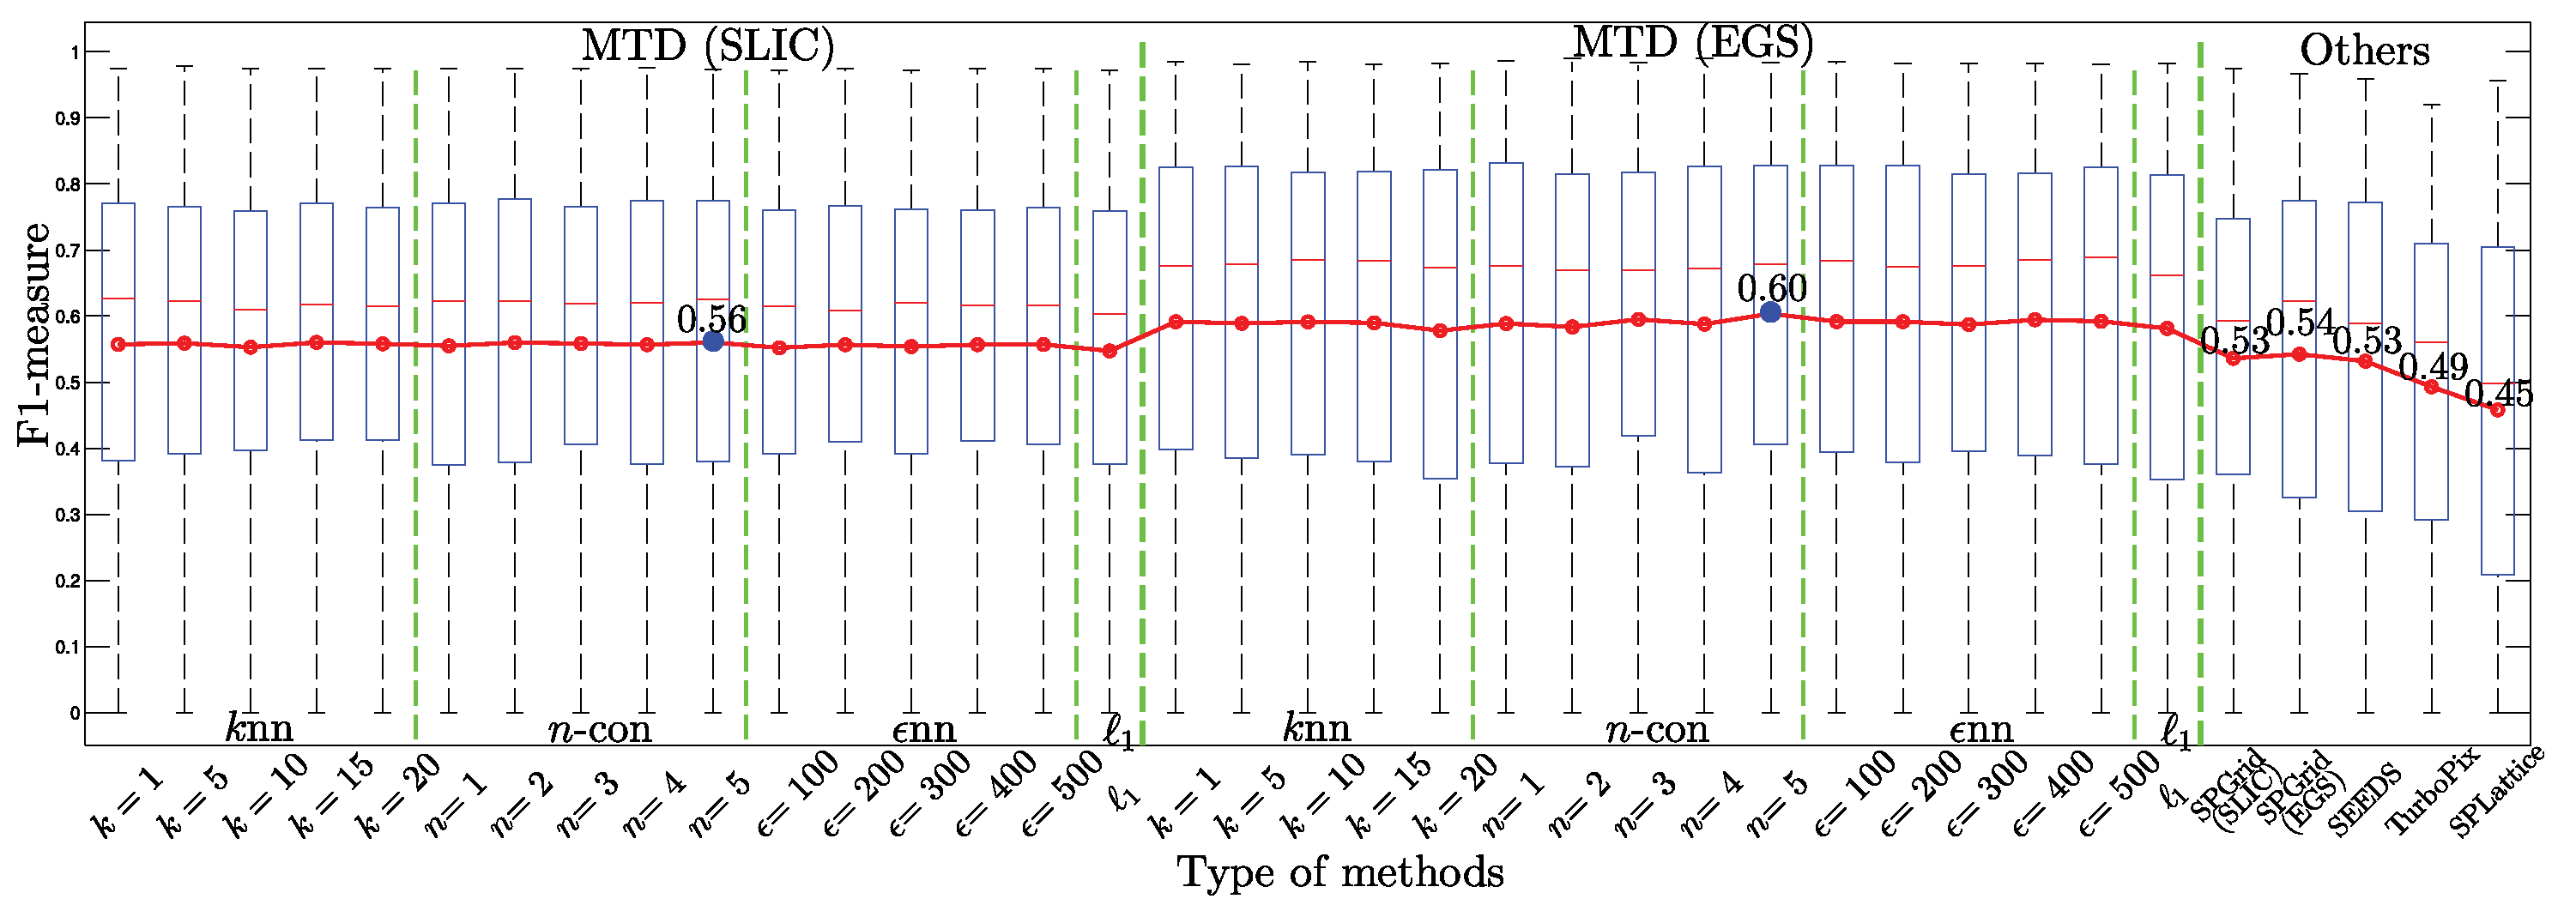
\includegraphics[width=\linewidth]{figs/de.eps}
\caption{$F1$-measures of 32 sub-variants of MTD and 5 state-of-the-art methods with DE optimized parameters.}
\label{fig:comp}
\end{figure*}
The right part of Fig.~\ref{fig:comp} plots the $F_1$-measure of all object localization methods. As for state-of-the-art methods, our previous SPGrid achieves similar performance to SEEDS (around 0.53). It is worthy pointing out that SPGrid-EGS is slightly better than SPGrid-SLIC, which is consistent with MTD variants. In comparison, TurboPixel gets a lower average $F_1$-measure (0.49), followed by SPLattice (0.45 on average). More importantly,  our MTD variants outperforms all the above methods with apparent improvements. The maximum $F_1$-measure is reported to be 0.56 and 0.60 for $n$-con MTD-SLIC and $n$-con MTD-EGS respectively.

\subsubsection{Robustness to image scaling, rotation and noise.}
We then evaluate the robustness of all methods to three disturbing factors, \ie noise, scale variation and rotation. For each factor, we consider 10 disturbing levels w.r.t. additive Gaussian noise variance, scale value and rotation degree, respectively, as showed in the horizontal axis of Fig.\ref{fig:robust}. Thus, we can build 30 datasets in total for three factors by transforming all the test cases w.r.t different disturbing levels. Then, we evaluate all methods on each dataset with the DE optimized parameters used in Fig.~\ref{fig:comp} and calculate the average $F1$-measure, as showed in Fig.~\ref{fig:robust}. Note that, since MTD variants with different graph types have similar performance, we calculate the average $F1$-measure of MTD-SLIC and MTD-EGS across all graphs,respectively.

As demonstrated in Fig.~\ref{fig:robust}, pixel-level RC is highly sensitive to noise and image scaling, and it drops quickly and consistently when the noise variance increases or the scaling factor decreases. TurboPixel, SPLattice, and SEEDS have similar performance when considering image noise. However, TurboPixel and SPLattice are sensitive to image rotation and have low $F_1$-measure similar to that of pixel-level RC. It is interesting to point out that SEEDS are robust to image scaling and rotation, and it have even improved $F_1$-measure when the scaling factor drops from 0.78 to 0.56.

In comparison, our MTD methods and previous SPGrid methods are more stable under varying image scaling factors, rotation, and noise corruptions. Futhermore, MTD-EGS achieves the best performance.
\begin{figure*}[ht]
\centering
\includegraphics[width=0.95\linewidth]{figs/robust.eps}
\caption{Robustness to scaling, rotation and noise for pixel-level RC, SPLattic, SEEDS, TurboPixle, SPGrid and our two MTD variants,\ie MTD-SLIC and MTD-EGS.}\label{fig:robust}
\end{figure*}

\subsubsection{Visual comparison} The visual comparison among different methods is presented in Fig.~\ref{fig:visual}. Note that, the results come from previous quantitative evaluation in subsection~\ref{subsec:compquant} with optimal parameters. For our MTD methods, as MTD with different SP graphs have similar performance, we just show the results of MTD-SLIC and MTD-EGS based on $n$-con graph. Both the $F_1$-measure and the whole timing are marked in each result. The leftmost of Fig.~\ref{fig:visual} shows the inputs of each case, \ie an image with a mask indicating the target object. The rest parts of Fig.~\ref{fig:visual} shows the retrieval results on another image with different methods.

Pixel-based RC returns rectangular matched regions, which covers only a part of objects under retrieval. SPLattice, TurboPixel, SEEDS have similar localization results in many cases, yet they are not able to well grasp the object boundary. SPGrid-SLIC and SPGrid-EGS can capture most of the object boundary with some background included and foreground lost. Obviously, MTD methods (both SLIC-based and EGS-based) improve our previous SPGrid methods. Let us take the last third and fourth image for example. The man can be identified with a complete boundary using MTD methods, yet miss some parts using SPGrid. The similar performance is shown in the dog case. We can also see that MTD-EGS gets more complete object boundaries than MTD-SLIC, for instance, the eagle in the last image.
\begin{figure*}[]
\centering
\includegraphics[width=\linewidth]{figs/visual.eps}
\caption{Visual comparison between different methods.}\label{fig:visual}
\end{figure*}

\begin{table*} [ht]
\begin{center}
\begin{tabular}{|l||c|c|c|c|c|c|c|}
\hline
Method & Precision & Recall & $F_1$ & Precom-Time(sec) & SP-Time(sec) & Matching-Time(sec) & Total-Time(sec)\\
\hline\hline
MTD $k$nn 3          & 0.59 & 0.60 & 0.59 & -    & 0.06 & 0.20 & 0.26    \\
\hline				
MTD $n$-con 5        & 0.63 & 0.57 & 0.60 & -    & 0.07 & 0.24 & 0.31    \\
\hline				
MTD $\epsilon$nn 400 & 0.61 & 0.58 & 0.59 & -    & 0.06 & 0.22 & 0.28    \\
\hline				
MTD $L_1$-graph      & 0.65 & 0.55 & 0.58 & -    & 0.06 & 0.92 & 0.98    \\
\hline				
SPGrid-SLIC       & 0.61 & 0.48 & 0.53 & -    & 0.16 & 0.24 & 0.40    \\
\hline				
SPGrid-EGS        & 0.64 & 0.50 & 0.54 & -    & 0.06 & 0.25 & 0.31    \\
\hline
SEEDS                & 0.62 & 0.50 & 0.53 & -    & 0.10 & 0.25 & 0.35    \\
\hline				
TurboPixel           & 0.61 & 0.44 & 0.49 & -    & 3.58 & 0.25 & 3.83    \\
\hline				
SPLattice            & 0.57 & 0.42 & 0.45 & 0.17 & 0.19 & 0.29 & 0.48    \\
\hline				
Pixel                & 0.40 & 0.61 & 0.42 & -    & -    & 7.38 & 7.38    \\
\hline
\end{tabular}
\end{center}
\caption{Average accuracy and speed of object localization using region covariance ~\cite{ol:tuzel06} on our extended MFC dataset.} \label{tab:allresults} \vspace{-0.3cm}
\end{table*}
%-------------------------------------------------------------------------
\section{Conclusion and Future Work}

{\small
\bibliographystyle{ieee}
\bibliography{spgrid_mtd_j}
}
\end{document}


